 \subsubsection{Passive 2-Tore} \label{subsubsec:2tore}
  
Passive 2-Tore sind Netzwerke mit 2 Klemmenpaaren, welche in jedem Betriebszustand Leistung verbrauchen. Ein Klemmenpaar wird auch als Tor bezeichnet. Dabei wird ein Tor als Eingang für ein Elektrisches Signal verwendet. Folglich wird am anderen Tor das Ausgangssignal abgegriffen. Ein Netzwerk, welches intern nur aus beliebigen R-(ohmischer Widerstand), L-(Induktivität), C-(Kapazität) und M-(Gegeninduktivität) Komponenten aufgebaut ist, ist immer ein passives Netzwerk. 

\begin{figure}[H]
	\centering
	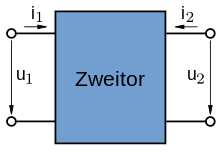
\includegraphics[width=5cm]{2Tor.png}
	\label{fig:2tor}
\end{figure}

Ein solches Netzwerk ist zusätzlich noch Reziprok. Reziproke Netzwerke haben die Eigenschaft, dass es egal ist, in welcher Richtung sie betrieben werden, solange der Innenwiderstand der Quelle gleich gross ist wie die Lastimpedanz. Anhand vom folgenden Beispiel wird dies veranschaulicht. Die Leistung im Verbraucher ist in beiden Betriebszuständen dieselbe. Diese Eigenschaft kann in der Praxis grosse Erleichterungen beim berechnen zur folge haben.

\begin{figure}[H]
	\centering
	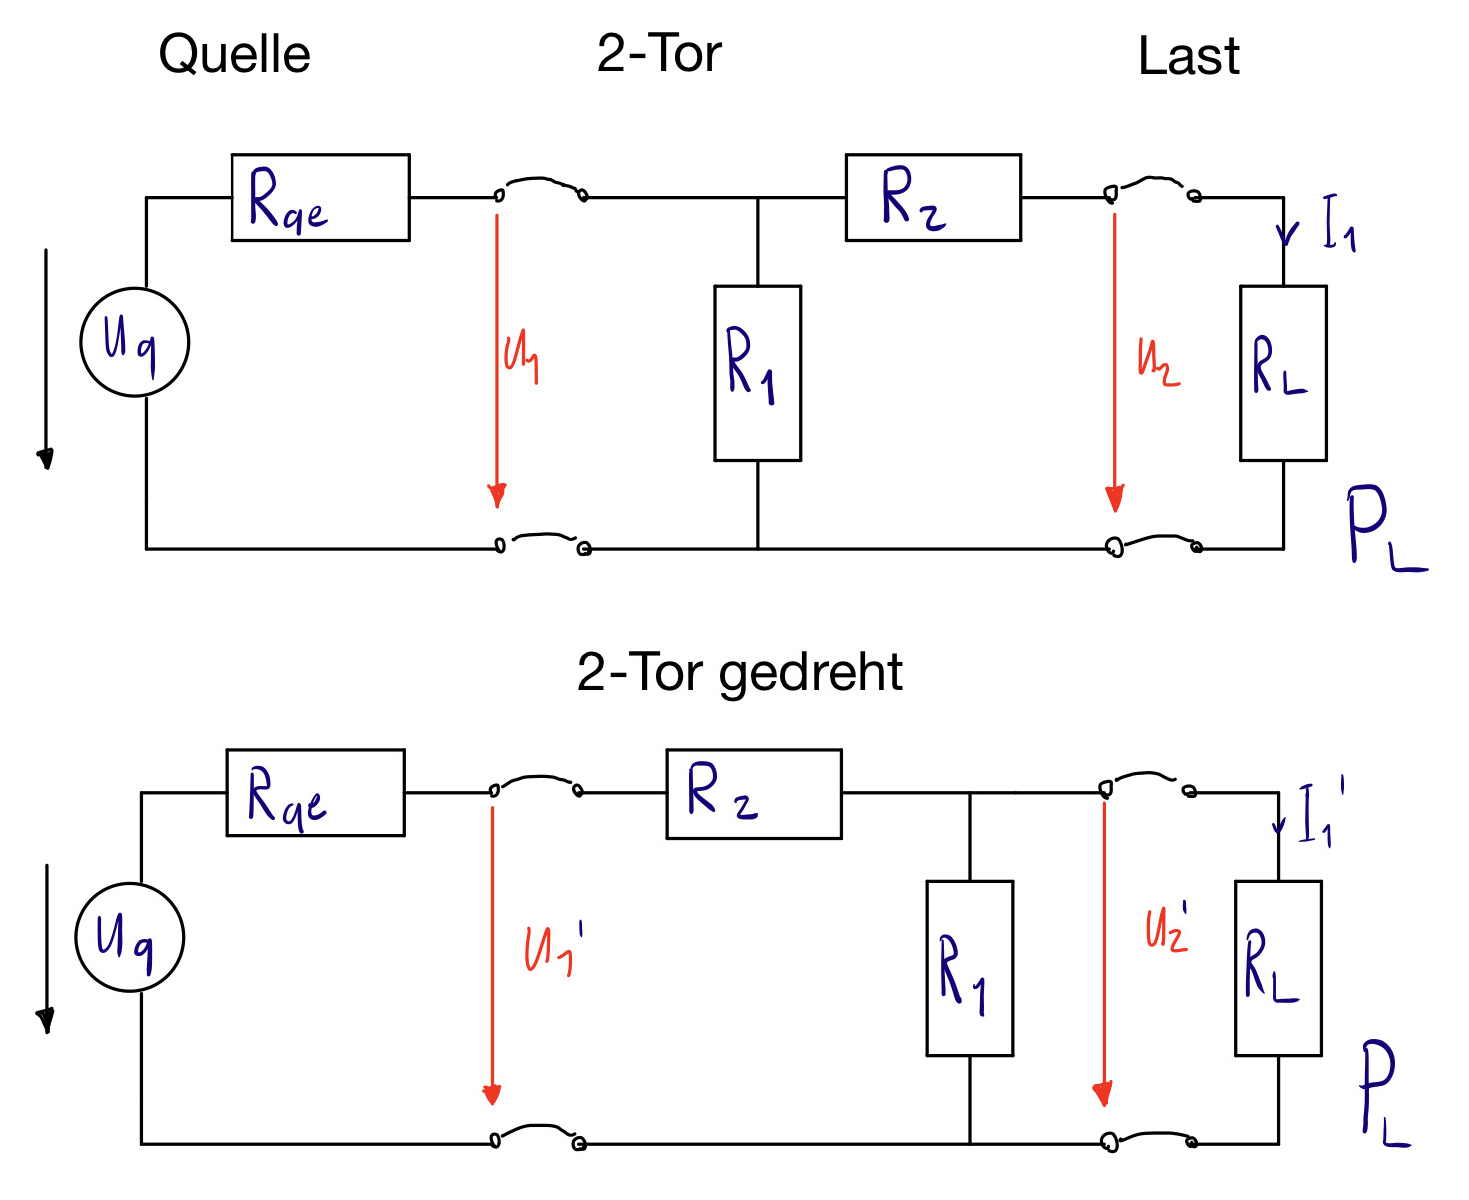
\includegraphics[width=12cm]{bsp_reziprok.jpg}
	\label{fig:reziprozitat}
\end{figure}


Seien R$_Q$ und R$_L$ jeweils 50 Ohm, R$_1$ 150 Ohm und R$_2$ 20 Ohm. Die Quelle liefert eine Spannung von 100V.

In beiden Netzwerken berechnen wir aus der Quelle und dem 2-Tor den Ersatzwiderstand.


\begin{equation}\label{equ:rqe1}
			R_{Q1} = \frac{1}{\frac{1}{R_Q}+\frac{1}{R_1}} +R_2 =  
		\end{equation}
und 
\begin{equation}\label{equ:rqe1}
			R_{Q2} = \frac{1}{\frac{1}{R_Q+R_2}+\frac{1}{R_1}} =  
		\end{equation}
		


\begin{figure}[H]
	\centering
	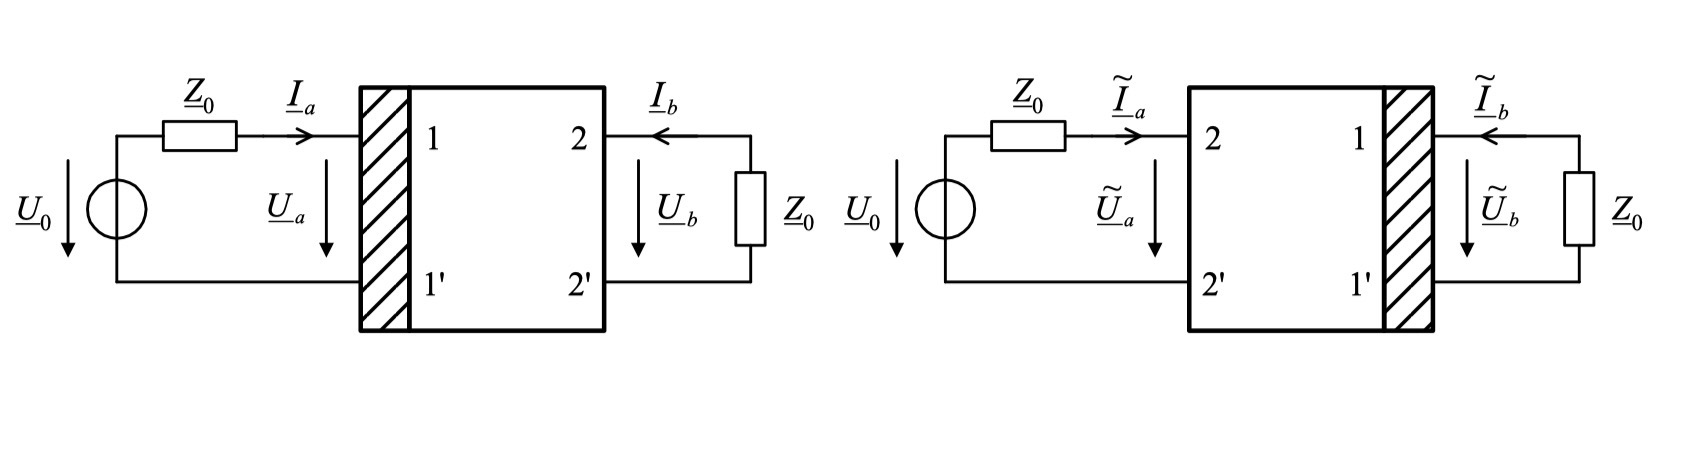
\includegraphics[width=12cm]{reziprozitat.jpg}
	\label{fig:reziprozitat}
\end{figure}

Im dargestellten Netzwerk gilt somit

\begin{equation}\label{equ:verticImpedance}
			\underline{I}_b =  \underline{\tilde{I}}_b
		\end{equation}
		
sowie 		
		
\begin{equation}\label{equ:verticImpedance}
			\underline{U}_b =  \underline{\widetilde{U}}_b
		\end{equation}

\newpage


